\section{Radds存储系统详细设计与实现}

	本章对存储系统的各层进行详细设计与实现,针对各层内部的子系统,各层之间的接口进行详细定义。

  \subsection{基础层详细设计与实现}
	
   	\subsubsection{错误处理的实现}

		针对go语言本身的特性,错误处理成为整个系统程序开发的首要项目,我们以轻量化,插件化的形式进行错误处理。
		
		\begin{lstlisting}[caption=Errors , label=code_radds_errors]

 
		\end{lstlisting}                 

	
			
   	\subsubsection{日志系统的实现}
    
	   为了防止写入内存的数据库因为进程异常、操作系统掉电等情况发生丢失,
	   存储系统在写内存之前会将本次写操作的内容写入日志文件中。
    
    \begin{figure}[H]
    	\centering
    	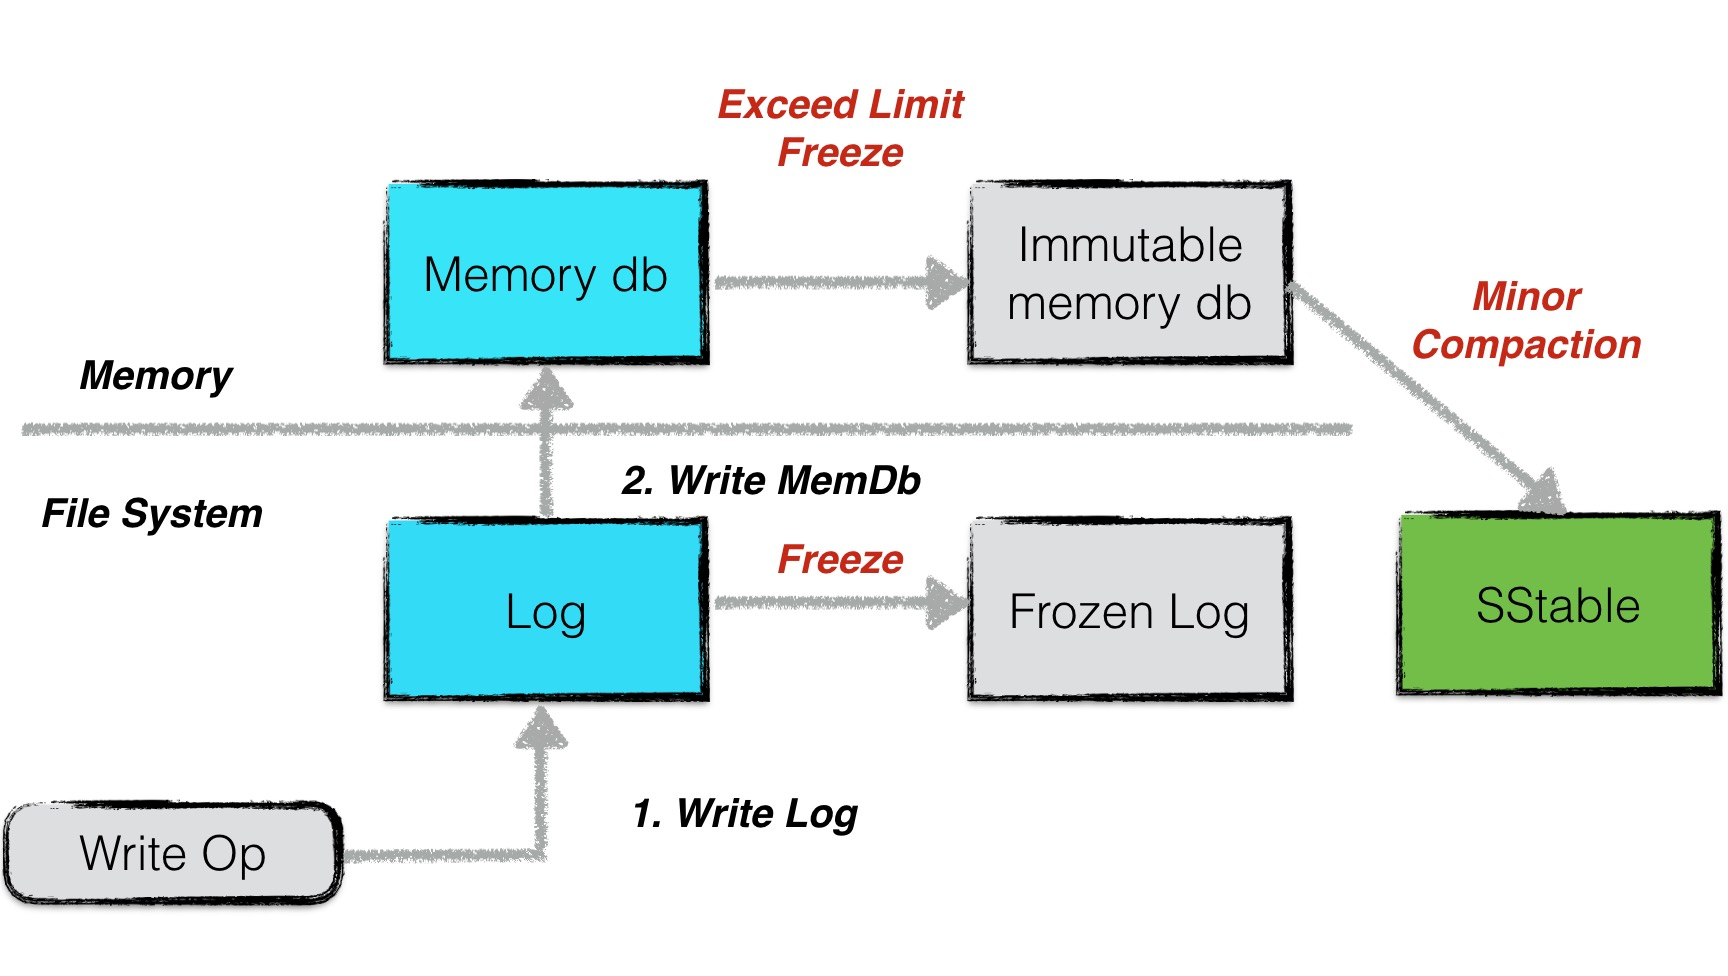
\includegraphics[width=0.95\textwidth]{images/two_log}
    	\caption{日志系统架构图}
    	\label{two_log}
    \end{figure}
	存储系统中,有两个memory db,以及对应的两份日志文件。
	其中一个memory db是可读写的,当这个db的数据量超过预定的上限时,
	便会转换成一个不可写的memory db,与此同时,与之对应的日志文件也变成一份frozen log。

	而新生成的immutable memory db则会由后台的minor compaction进程将其转换成一个sstable文件进行持久化,
	持久化完成,与之对应的frozen log被删除。
    
	\begin{enumerate}
		\item 日志结构

		\begin{figure}[H]
			\centering
			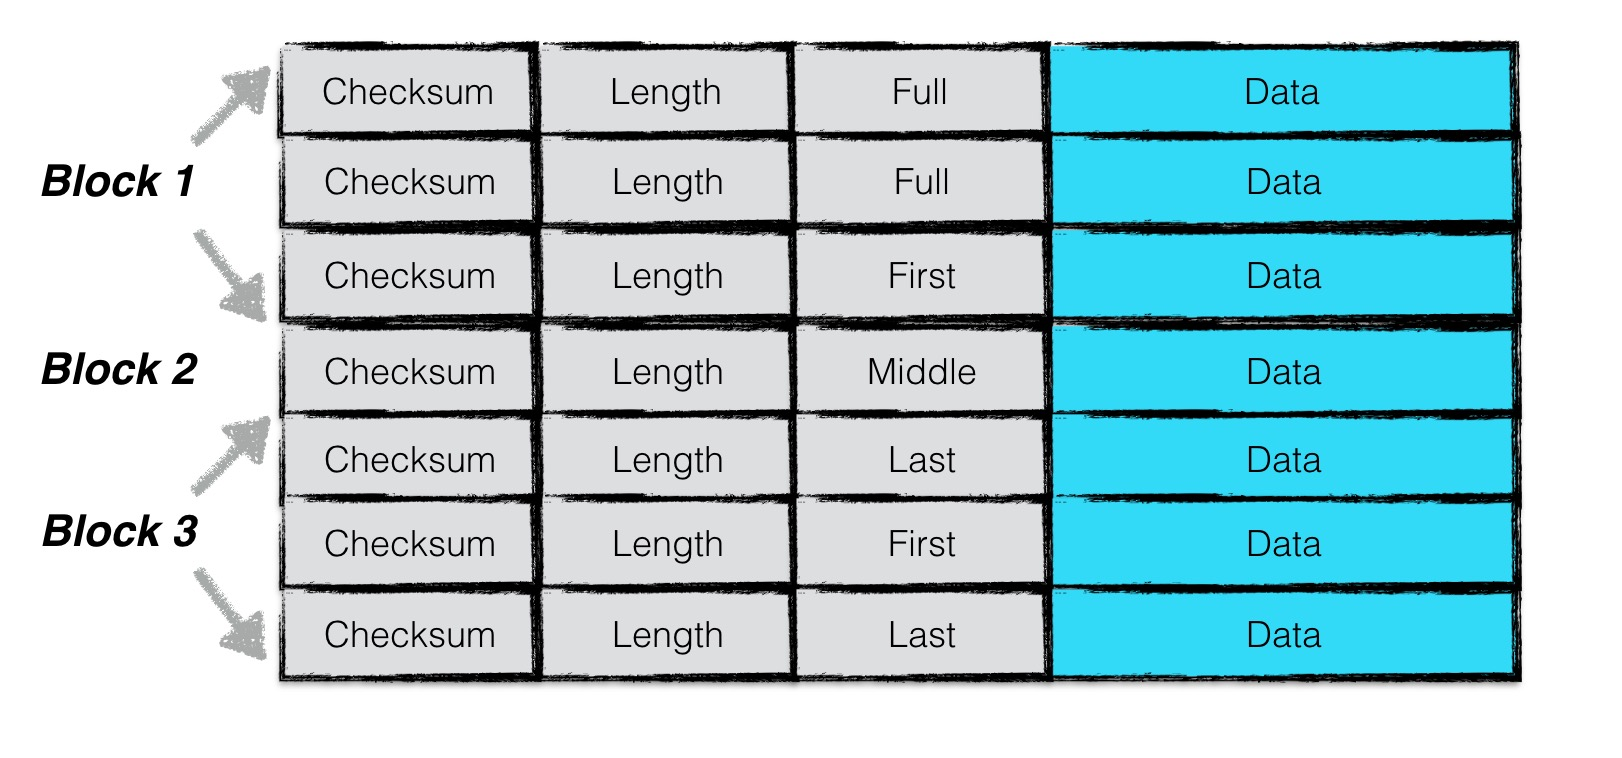
\includegraphics[width=0.95\textwidth]{images/journal}
			\caption{日志文件存储结构图}
			\label{journal}
		\end{figure}
		为了增加读取效率,日志文件中按照block进行划分,每个block的大小为32KiB。
		每个block中包含了若干个完整的chunk。
		
		一条日志记录包含一个或多个chunk。
		每个chunk包含了一个7字节大小的header,前4字节是该chunk的校验码,
		紧接的2字节是该chunk数据的长度,以及最后一个字节是该chunk的类型。
		其中checksum校验的范围包括chunk的类型以及随后的data数据。
	
		chunk共有四种类型:full,first,middle,last。
		一条日志记录若只包含一个chunk,则该chunk的类型为full。
		若一条日志记录包含多个chunk,则这些chunk的第一个类型为first, 
		最后一个类型为last,中间包含大于等于0个middle类型的chunk。
		
		由于一个block的大小为32KiB,因此当一条日志文件过大时,
		会将第一部分数据写在第一个block中,且类型为first,
		若剩余的数据仍然超过一个block的大小,则第二部分数据写在第二个block中,
		类型为middle,最后剩余的数据写在最后一个block中,类型为last。
		
		\item 日志内容
		
		日志的内容为写入的batch编码后的信息。

		具体的格式为:

		\begin{figure}[H]
			\centering
			
\includegraphics[width=0.95\textwidth]{images/journal_content}
			\caption{日志文件格式图}
			\label{journal_content}
		\end{figure}

		一条日志记录的内容包含:Header和Data
		其中Header中有(1)当前db的sequence number(2)本次日志记录中所包含的put/del操作的个数。
		
		紧接着写入所有batch编码后的内容。
		\item 日志文件写 
		
		\begin{figure}[H]
			\centering
			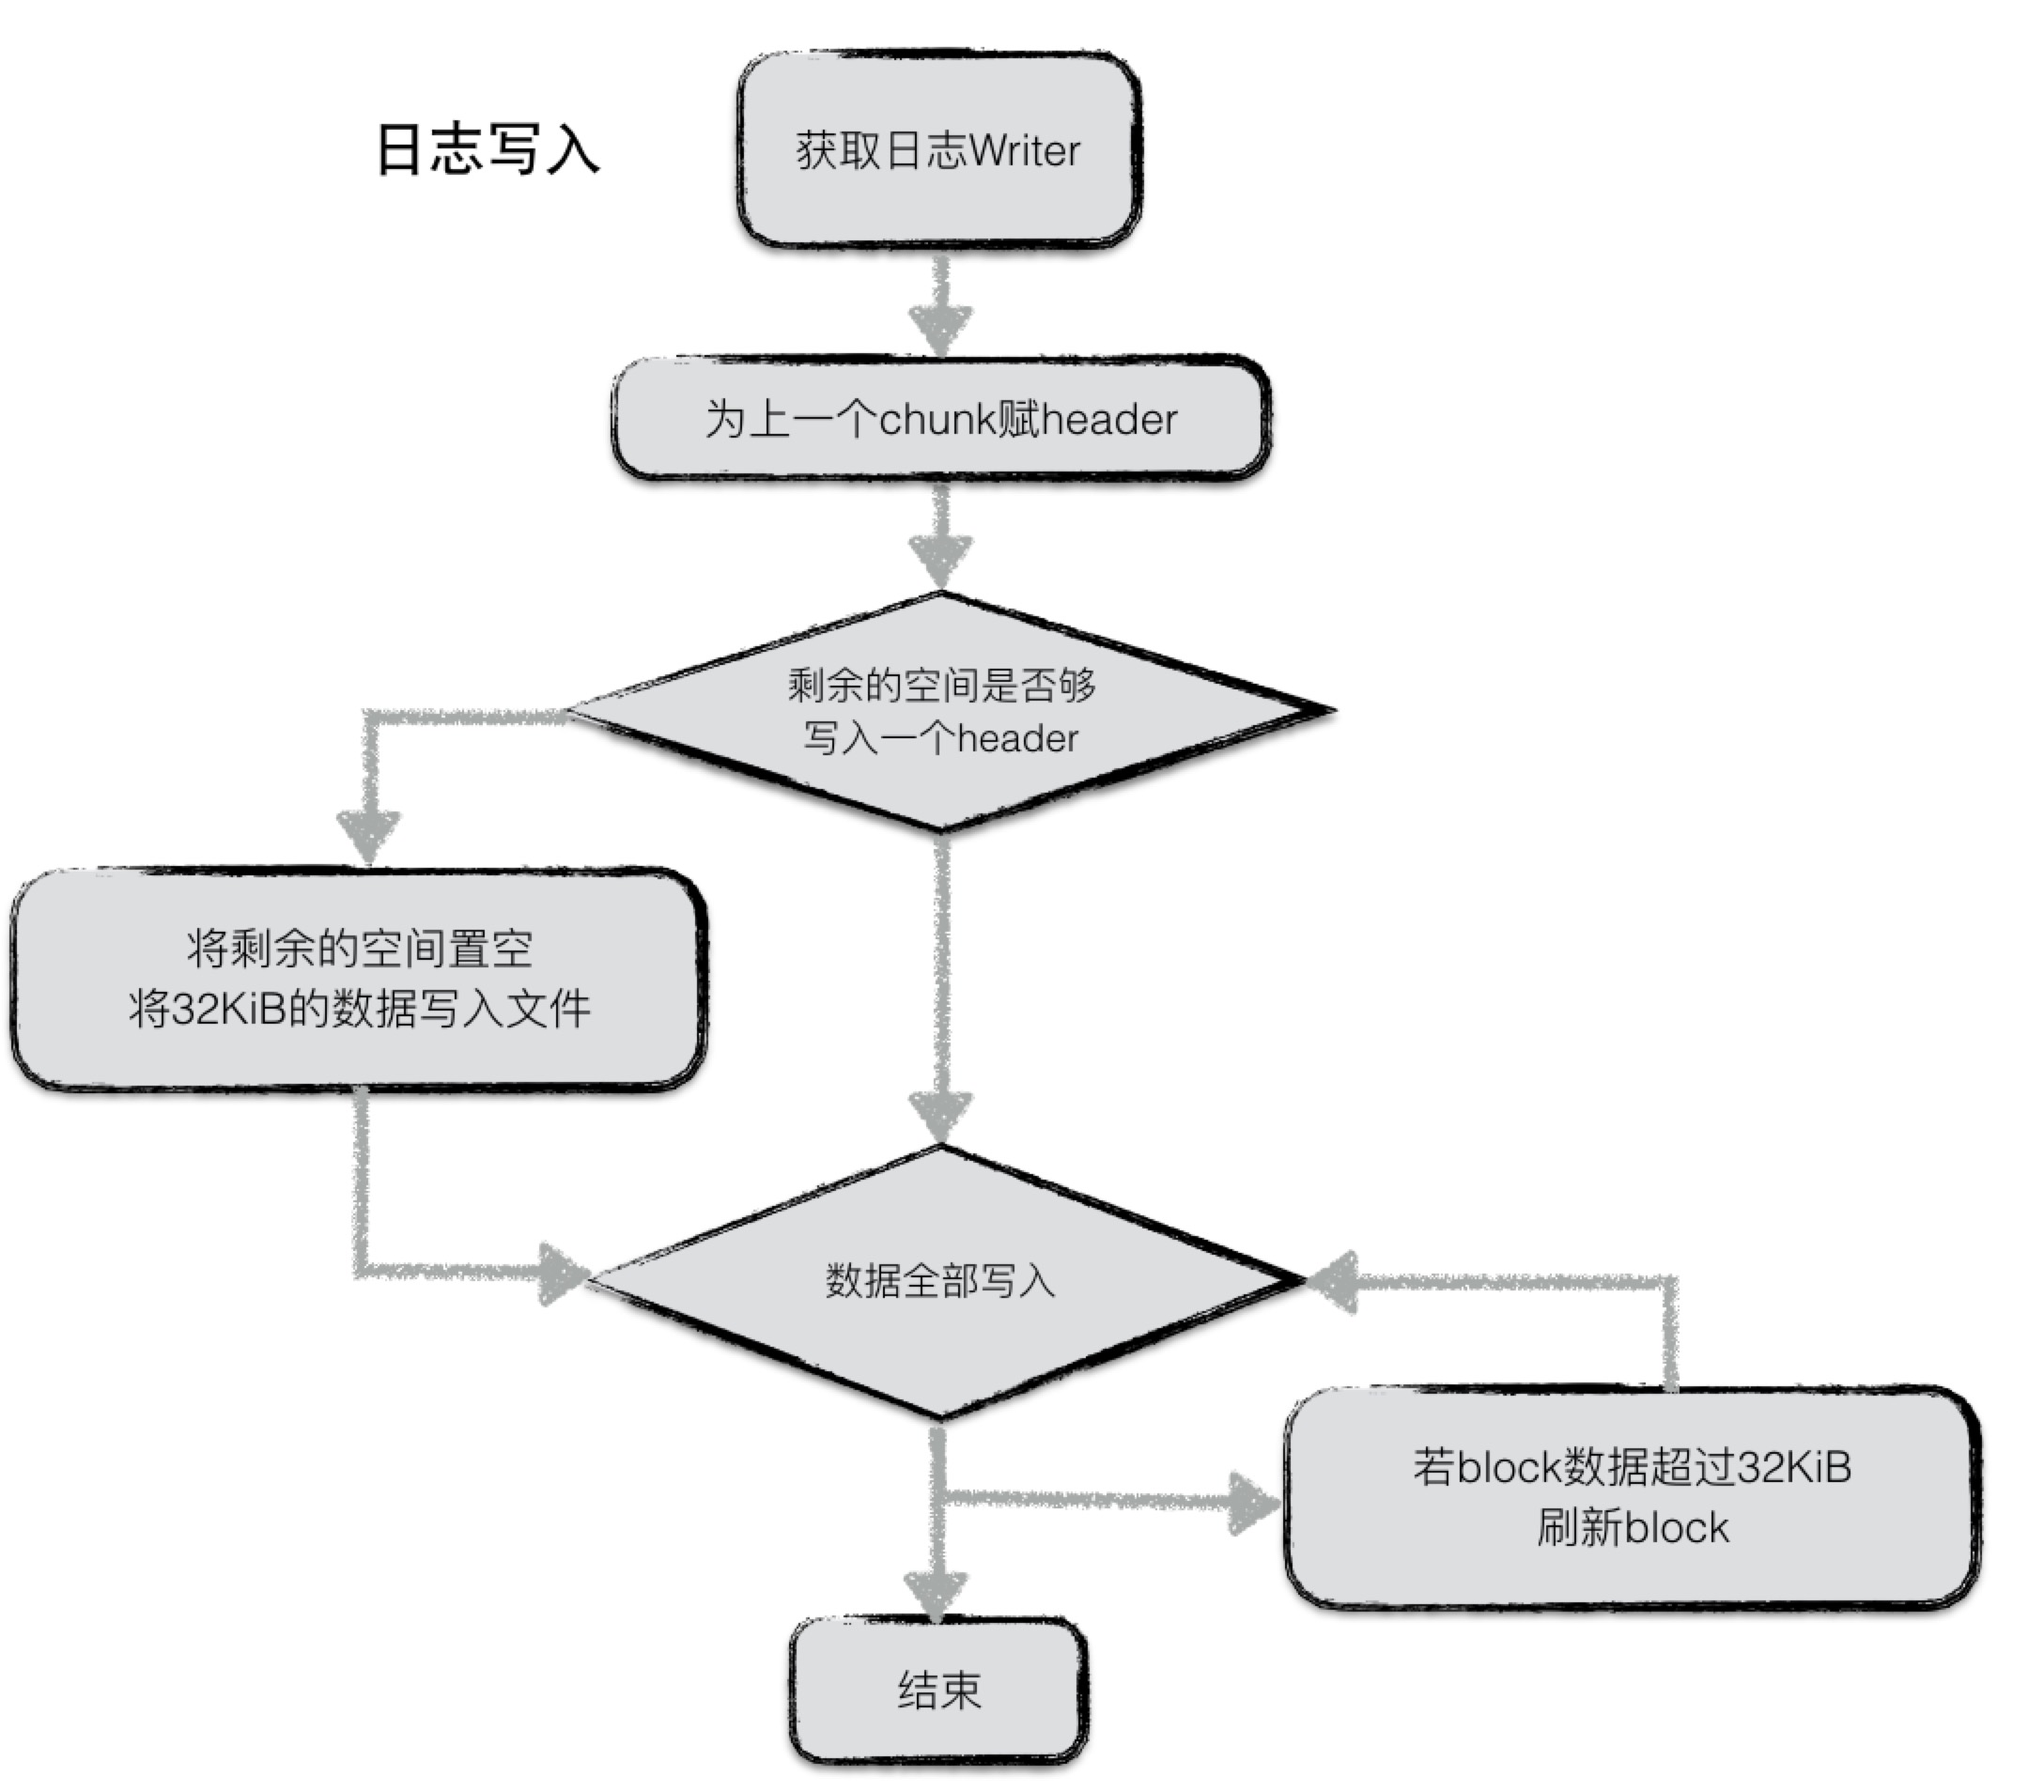
\includegraphics[width=0.95\textwidth]{images/journal_write}
			\caption{日志文件写流程图}
			\label{journal_write}
		\end{figure}
		
		日志写入流程较为简单,在存储系统内部,实现了一个journal的writer。
		首先调用Next函数获取一个singleWriter,
		这个singleWriter的作用就是写入一条journal记录。

		singleWriter开始写入时,标志着第一个chunk开始写入。
		在写入的过程中,不断判断writer中buffer的大小,若超过32KiB,
		将chunk开始到现在做为一个完整的chunk,为其计算header之后将整个chunk写入文件。
		与此同时reset buffer,开始新的chunk的写入。

		若一条journal记录较大,则可能会分成几个chunk存储在若干个block中。

		\item 日志文件读 
		
		同样,日志读取也较为简单。为了避免频繁的IO读取,每次从文件中读取数据时,
		按block(32KiB)进行块读取。

		每次读取一条日志记录,reader调用Next函数返回一个singleReader。
		singleReader每次调用Read函数就返回一个chunk的数据。每次读取一个chunk,
		都会检查这批数据的校验码、数据类型、数据长度等信息是否正确,若不正确,
		且用户要求严格的正确性,则返回错误,否则丢弃整个chunk的数据。

		循环调用singleReader的read函数,直至读取到一个类型为Last的chunk,
		表示整条日志记录都读取完毕,返回。

		\begin{figure}[H]
			\centering
			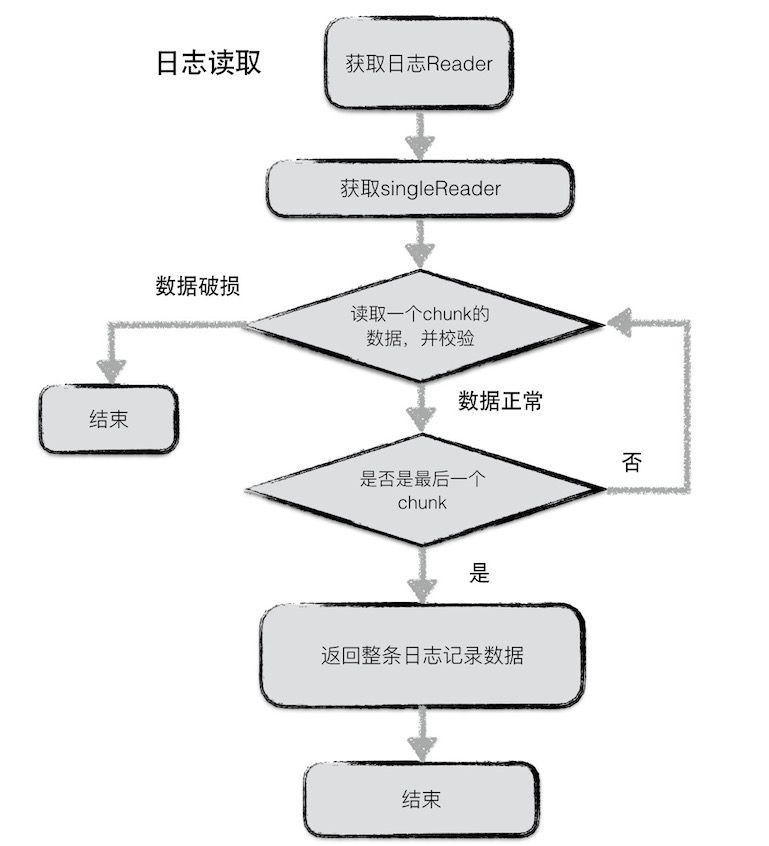
\includegraphics[width=0.95\textwidth]{images/journal_read}
			\caption{日志文件读流程图}
			\label{journal_read}
		\end{figure}
		
		
	
	\end{enumerate}
	
   	\subsubsection{工具库的实现}
    


  	\subsection{存储层详细设计与实现}
	

	
  	\subsection{共识层详细设计与实现}


        

  \subsection{客户端层详细设计与实现}
  	
		\subsubsection{API 客户端服务平台的实现}
		
		
		\subsubsection{gRPC API客户端的实现}
		
		
	 	\subsubsection{RESTful API客户端的实现}
	 	
	 	
		\subsubsection{CLI 命令行客户端的实现}
		


	\subsection{本章小结}
 \clearpage